\newpage
\section{Teilversuch 5: Bestätigung der Kirchhoffschen Sätze}
	Versuchsaufbau:
	\begin{center}
		\vfill
		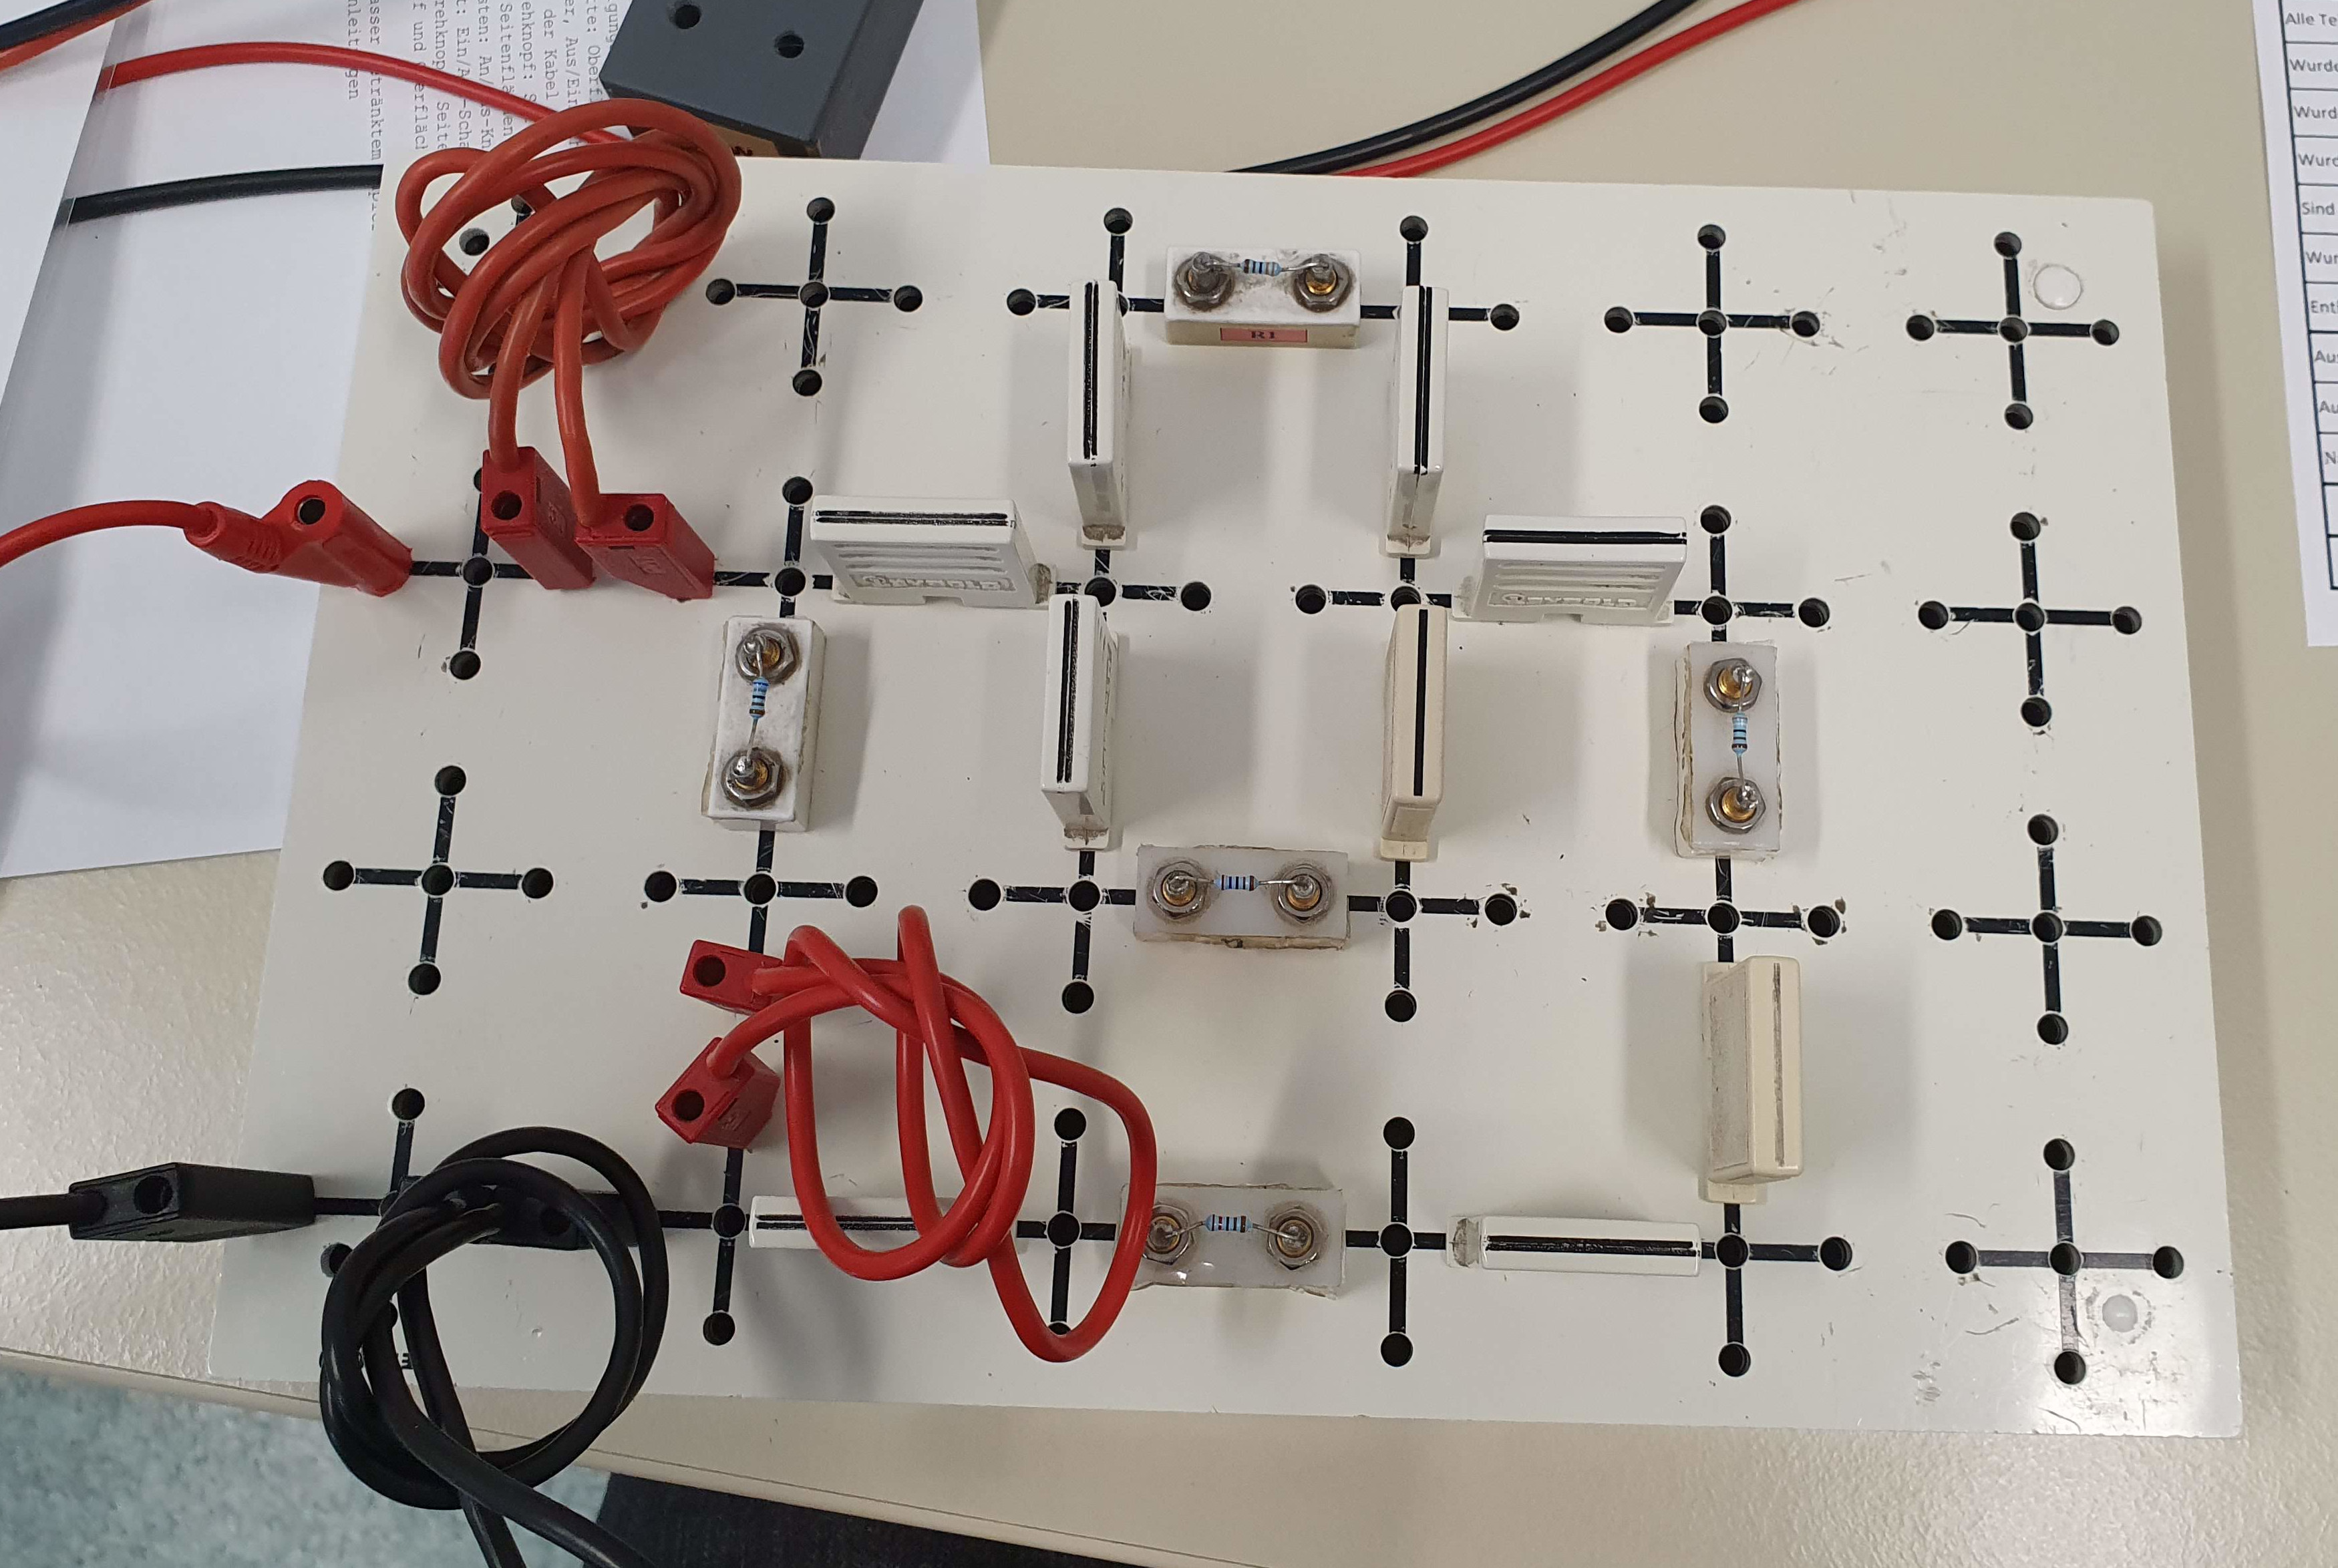
\includegraphics[width=0.7\textwidth]{versuchsaufbau-tv5.jpg}
		\vfill
	\end{center}
	\begin{multicols}{2}
		\begin{center}
			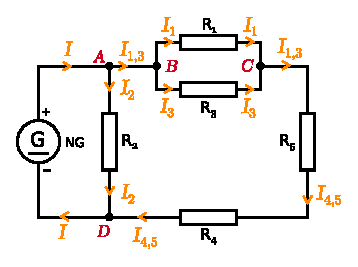
\includegraphics{tv5-junctions.eps}
		\end{center}
		\begin{equation*}
			\begin{tabu}{ll}
				\toprule
				I & \SI{2.70(13)}{\milli\ampere}\\
				I_1 & \SI{0.60(11)}{\milli\ampere}\\
				I_2 & \SI{1.40(12)}{\milli\ampere}\\
				I_3 & \SI{0.70(11)}{\milli\ampere}\\
				I_{4,5} & \SI{1.30(12)}{\milli\ampere}\\
				I_{1,3} & \SI{1.30(12)}{\milli\ampere}\\
				\bottomrule
			\end{tabu}
		\end{equation*}
	\end{multicols}
	\textbf{Knoten $A$}

	Es gilt aus der Knotenregel:
	\begin{align}
	 	S = I - I_{1,3}  - I_2 = 0 && \Delta S = \addquad{I, I_{1,3}, I_2}
	\end{align} 
	Nach Substitution:
	\begin{align*}
		S &= \SI{2.70}{\milli\ampere} - \SI{1.30}{\milli\ampere} - \SI{1.40}{\milli\ampere} = \SI{0}{\milli\ampere} \\
		\Delta S &= \addquad{\SI{0.13}{\milli\ampere}, \SI{0.12}{\milli\ampere}, \SI{0.12}{\milli\ampere}} = \SI{0.22}{\milli\ampere} \\
		\Rightarrow S &= \SI{0.00(22)}{\milli\ampere} 
	\end{align*}
	Also gilt die Knotenregel.

	\newpage
	\textbf{Knoten $B$}
	
	Es gilt aus der Knotenregel:
	\begin{align}
	 	S = I_{1,3}  - I_1 - I_3 = 0 && \Delta S = \addquad{I_{1,3}, I_1, I_3}
	\end{align} 
	Nach Substitution:
	\begin{align*}
		S &= \SI{1.30}{\milli\ampere} - \SI{0.60}{\milli\ampere} - \SI{0.70}{\milli\ampere} = \SI{0}{\milli\ampere} \\
		\Delta S &= \addquad{\SI{0.12}{\milli\ampere}, \SI{0.11}{\milli\ampere}, \SI{0.11}{\milli\ampere}} = \SI{0.20}{\milli\ampere} \\
		\Rightarrow S &= \SI{0.00(20)}{\milli\ampere} 
	\end{align*}
	Also gilt die Knotenregel.

	\textbf{Knoten $C$}
	
	Es gilt aus der Knotenregel:
	\begin{align}
	 	S = I_1 + I_3 - I_{1,3}  = 0 && \Delta S = \addquad{I_1, I_3, I_{1,3}}
	\end{align} 
	Nach Substitution:
	\begin{align*}
		S &= \SI{0.60}{\milli\ampere} + \SI{0.70}{\milli\ampere} - \SI{1.30}{\milli\ampere}= \SI{0}{\milli\ampere} \\
		\Delta S &= \addquad{\SI{0.11}{\milli\ampere}, \SI{0.11}{\milli\ampere}, \SI{0.12}{\milli\ampere}} = \SI{0.20}{\milli\ampere} \\
		\Rightarrow S &= \SI{0.00(20)}{\milli\ampere} 
	\end{align*}
	Also gilt die Knotenregel.

	\textbf{Knoten $D$}
	
	Es gilt aus der Knotenregel:
	\begin{align}
	 	S = I_2 + I_{4,5} - I  = 0 && \Delta S = \addquad{I_2, I_{4,5}, I}
	\end{align} 
	Nach Substitution:
	\begin{align*}
		S &= \SI{1.40}{\milli\ampere} + \SI{1.30}{\milli\ampere} - \SI{2.70}{\milli\ampere}= \SI{0}{\milli\ampere} \\
		\Delta S &= \addquad{\SI{0.12}{\milli\ampere}, \SI{0.12}{\milli\ampere}, \SI{0.13}{\milli\ampere}} = \SI{0.22}{\milli\ampere} \\
		\Rightarrow S &= \SI{0.00(22)}{\milli\ampere} 
	\end{align*}
	Also gilt die Knotenregel.


	\begin{multicols}{2}
		\begin{center}
			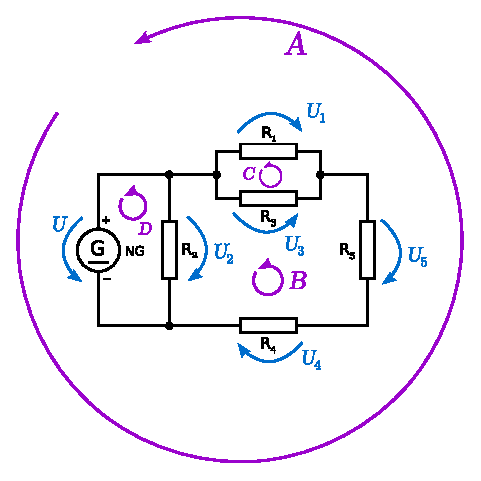
\includegraphics{tv5-loops.eps}
		\end{center}
		\begin{equation*}
			\begin{tabu}{ll}
				\toprule
				U & \SI{10.04(7)}{\volt}\\
				U_1 & \SI{1.974(11)}{\volt}\\
				U_2 & \SI{10.04(7)}{\volt}\\
				U_3 & \SI{1.974(11)}{\volt}\\
				U_4 & \SI{2.910(25)}{\volt}\\
				U_5 & \SI{5.16(4)}{\volt}\\
				\bottomrule
			\end{tabu}
		\end{equation*}
	\end{multicols}
	\textbf{Masche $A$}
	
	Es gilt aus der Maschenregel:
	\begin{align}
	 	S &= U - U_4 -U_5 - U_{1/3} = U - U_4 -U_5 - U_1 = 0\\ 
	 	\Delta S &= \addquad{U, U_4, U_5, U_1}
	\end{align} 
	Nach Substitution:
	\begin{align*}
		S &=  \SI{10.04}{\volt} - \SI{2.910}{\volt} - \SI{5.16}{\volt} - \SI{1.974}{\volt} = -\SI{0.004}{\volt}\\
		\Delta S &= \addquad{\SI{0.07}{\volt}, \SI{0.025}{\volt}, \SI{0.04}{\volt}, \SI{0.011}{\volt}} = \SI{0.09}{\volt} \\
		\Rightarrow S &= \SI{0.00(9)}{\volt} 
	\end{align*}
	Also gilt die Maschenregel.

	\textbf{Masche $B$}
	
	Es gilt aus der Maschenregel:
	\begin{align}
	 	S &= U_2 - U_4 -U_5 - U_{1/3} = U_2 - U_4 -U_5 - U_1 = 0 \\
	 	 \Delta S &= \addquad{U_2, U_4, U_5, U_1}
	\end{align} 
	Nach Substitution:
	\begin{align*}
		S &=  \SI{10.04}{\volt} - \SI{2.910}{\volt} - \SI{5.16}{\volt} - \SI{1.974}{\volt} = -\SI{0.004}{\volt}\\
		\Delta S &= \addquad{\SI{0.07}{\volt}, \SI{0.025}{\volt}, \SI{0.04}{\volt}, \SI{0.011}{\volt}} = \SI{0.09}{\volt} \\
		\Rightarrow S &= \SI{0.00(9)}{\volt} 
	\end{align*}
	Also gilt die Maschenregel.

	\textbf{Masche $C$}
	
	Es gilt aus der Maschenregel:
	\begin{align}
	 	S = U_3 - U_1 = 0 && \Delta S = \addquad{U_3, U_1}
	\end{align} 
	Nach Substitution:
	\begin{align*}
		S &=  \SI{1.974}{\volt} - \SI{1.974}{\volt} = \SI{0.000}{\volt}\\
		\Delta S &= \addquad{\SI{0.011}{\volt},\SI{0.011}{\volt}} = \SI{0.016}{\volt} \\
		\Rightarrow S &= \SI{0.000(16)}{\volt} 
	\end{align*}
	Also gilt die Maschenregel.

	\textbf{Masche $D$}
	
	Es gilt aus der Maschenregel:
	\begin{align}
	 	S = U - U_2 = 0 && \Delta S = \addquad{U, U_2}
	\end{align} 
	Nach Substitution:
	\begin{align*}
		S &=  \SI{10.04}{\volt} - \SI{10.04}{\volt} = \SI{0.00}{\volt}\\
		\Delta S &= \addquad{\SI{0.07}{\volt},\SI{0.07}{\volt}} = \SI{0.10}{\volt} \\
		\Rightarrow S &= \SI{0.00(10)}{\volt} 
	\end{align*}
	Also gilt die Maschenregel.
